\begin{figure}[h]
	\begin{center}
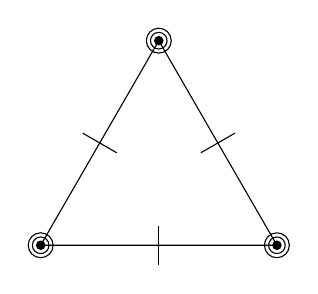
\begin{tikzpicture}[scale=0.5]
	%define the vertices of the triangle
	\path[coordinate] (0,0) coordinate(A)
		++(60:3cm) coordinate(D)
		++(60:3cm) coordinate(B)
		++(-60:3cm) coordinate(E)
		++(-60:3cm) coordinate(C)
		++(180:3cm) coordinate(F);
	%label the vertices and draw edges
	\draw (A) -- (D) -- (B) -- (E) -- (C) -- (F) -- cycle;
	%draw the interpolation points
	%function values
	\filldraw[black] (A) circle(3pt); 
	\filldraw[black] (B) circle(3pt); 
	\filldraw[black] (C) circle(3pt); 
	%first derivatives
	\draw[black] (A) circle(6pt); 
	\draw[black] (B) circle(6pt); 
	\draw[black] (C) circle(6pt); 
	%second derivatives
	\draw[black] (A) circle(9pt); 
	\draw[black] (B) circle(9pt); 
	\draw[black] (C) circle(9pt); 
	%normal derivatives
	\draw (1.067,2.848) -- (D) -- (1.933,2.348); 
	\draw (4.067,2.348) -- (E) -- (4.933,2.848); 
	\draw (3,-0.5cm) -- (F) -- (3,0.5cm); 
	%labels
%	\node[below of=A, node distance=0.5cm] (k) {$k=j+1$};
% \node[above of=B, node distance=0.5cm] (j) {$j=i+1$};
%	\node[below of=C, node distance=0.5cm] (i) {$i$};
\end{tikzpicture}
	\end{center}
	\caption{Argyris element with its 21 degrees of freedom.}
	\label{fig:Argyris}
\end{figure}
